\documentclass[12pt]{article}
\usepackage[margin=1.0in]{geometry}
\usepackage{graphicx}
\bibliographystyle{plain}
\usepackage{mathtools}
\usepackage{subfigure}

\begin{document}

\section{Specific Aim 2.1}

SET domain protein models of SETD2, NSD1, and NSD2 were built using Modeller with PDBs 4FMU, 3OOI, and 3OOI as inputs, respectively.  Proteins were surrounded by TIP3P boxes of approximately 7 nm, with NaCl ions added to achieve neutrality.  The ff99sb-ildn force field \cite{} was used.  Systems were held at constant temperature (300K) and pressure (1.01 atmospheres) using a Langevin integrator and Monte Carlo barostat, as implemented in OpenMM 5.5.1 \cite{}.  For each system, an aggregate of 10-20 $\mu$ s of simulations were analyzed using MDTraj, MSMBuilder \cite{}, and Mixtape \cite{}.  Slow coordinates were selected using temporal indendent component analysis (TICA) \cite{} with randomly selected distances as inputs.  Five-state Gaussian Hidden Markov Models were constructed in the basis of the two slowest linear combinations of features.  

\begin{figure}
\subfigure[]{
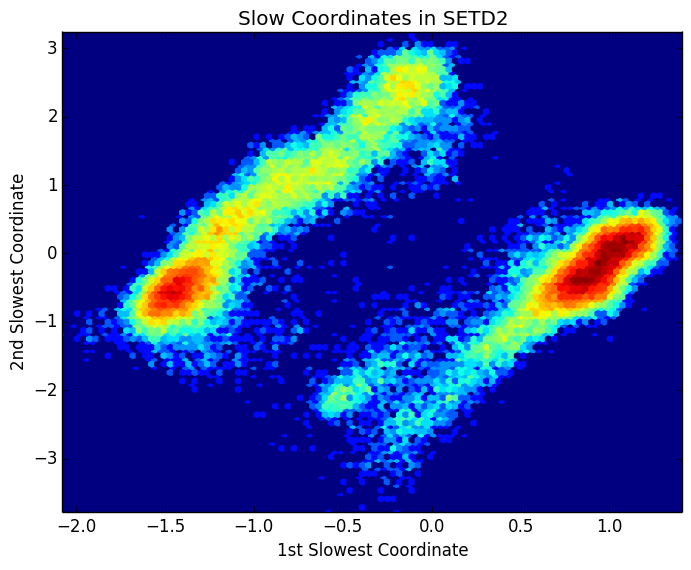
\includegraphics[width=5.5cm]{figures/SETD2_tics.png}
}
\subfigure[]{
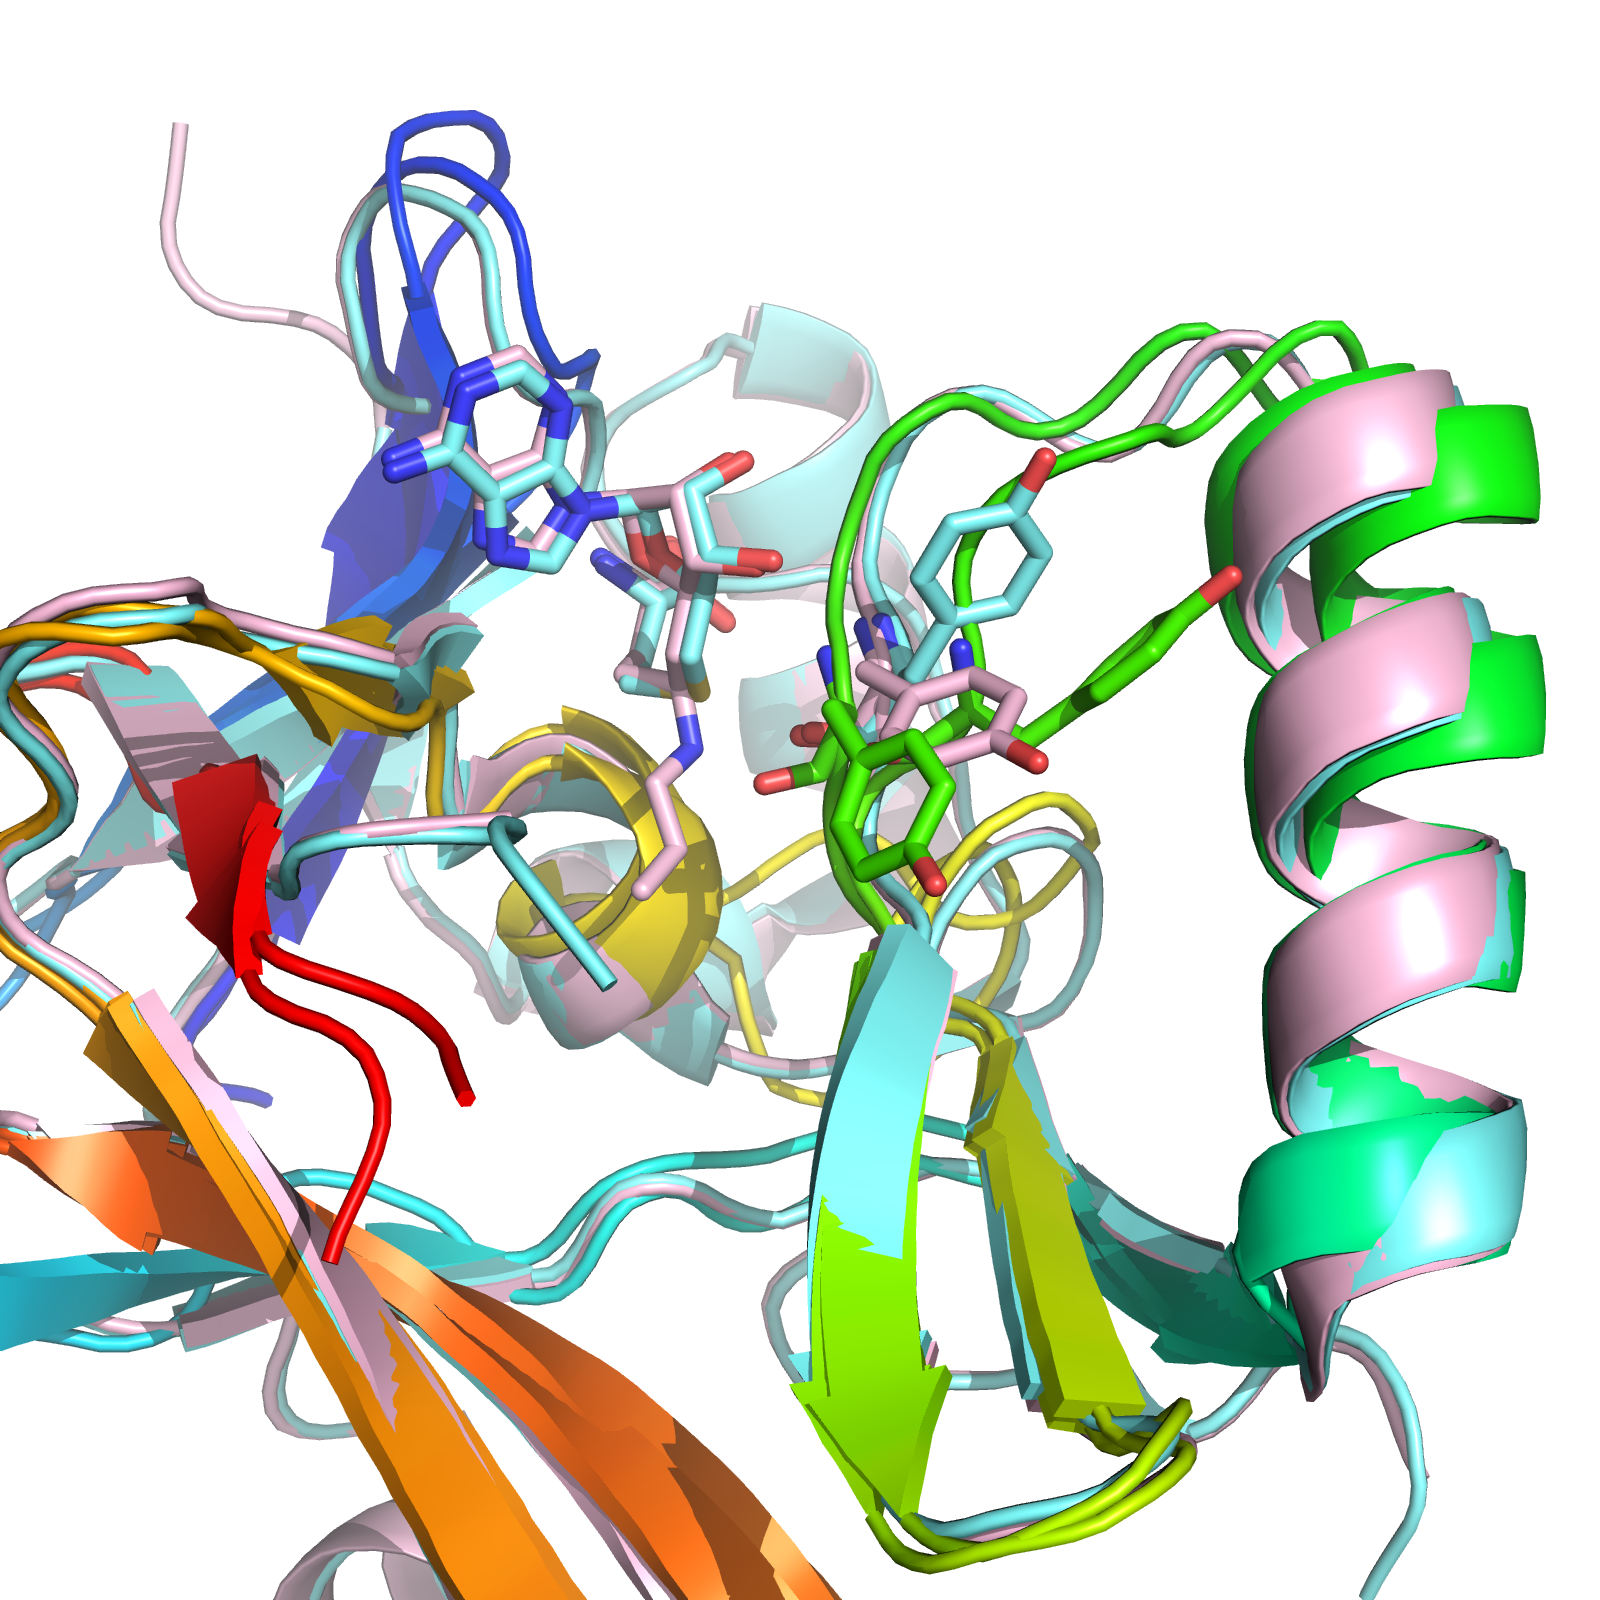
\includegraphics[width=5.5cm]{figures/SETD2_pdb.png}
}

\subfigure[]{
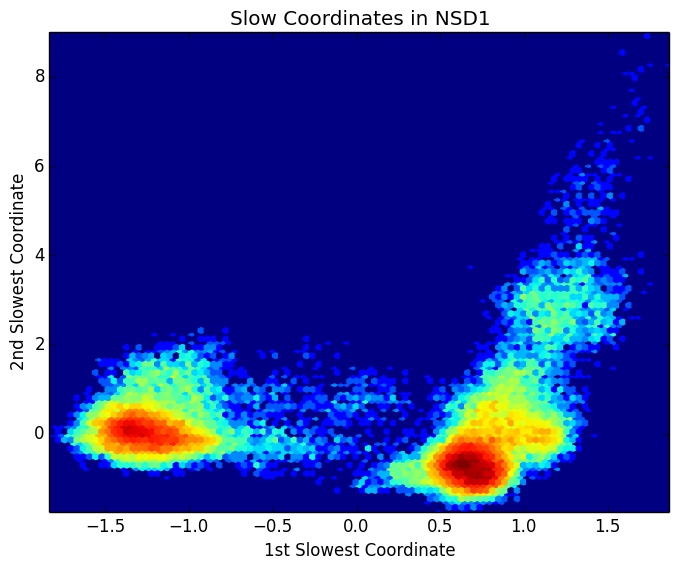
\includegraphics[width=5.5cm]{figures/NSD1_tics.png}
}
\subfigure[]{
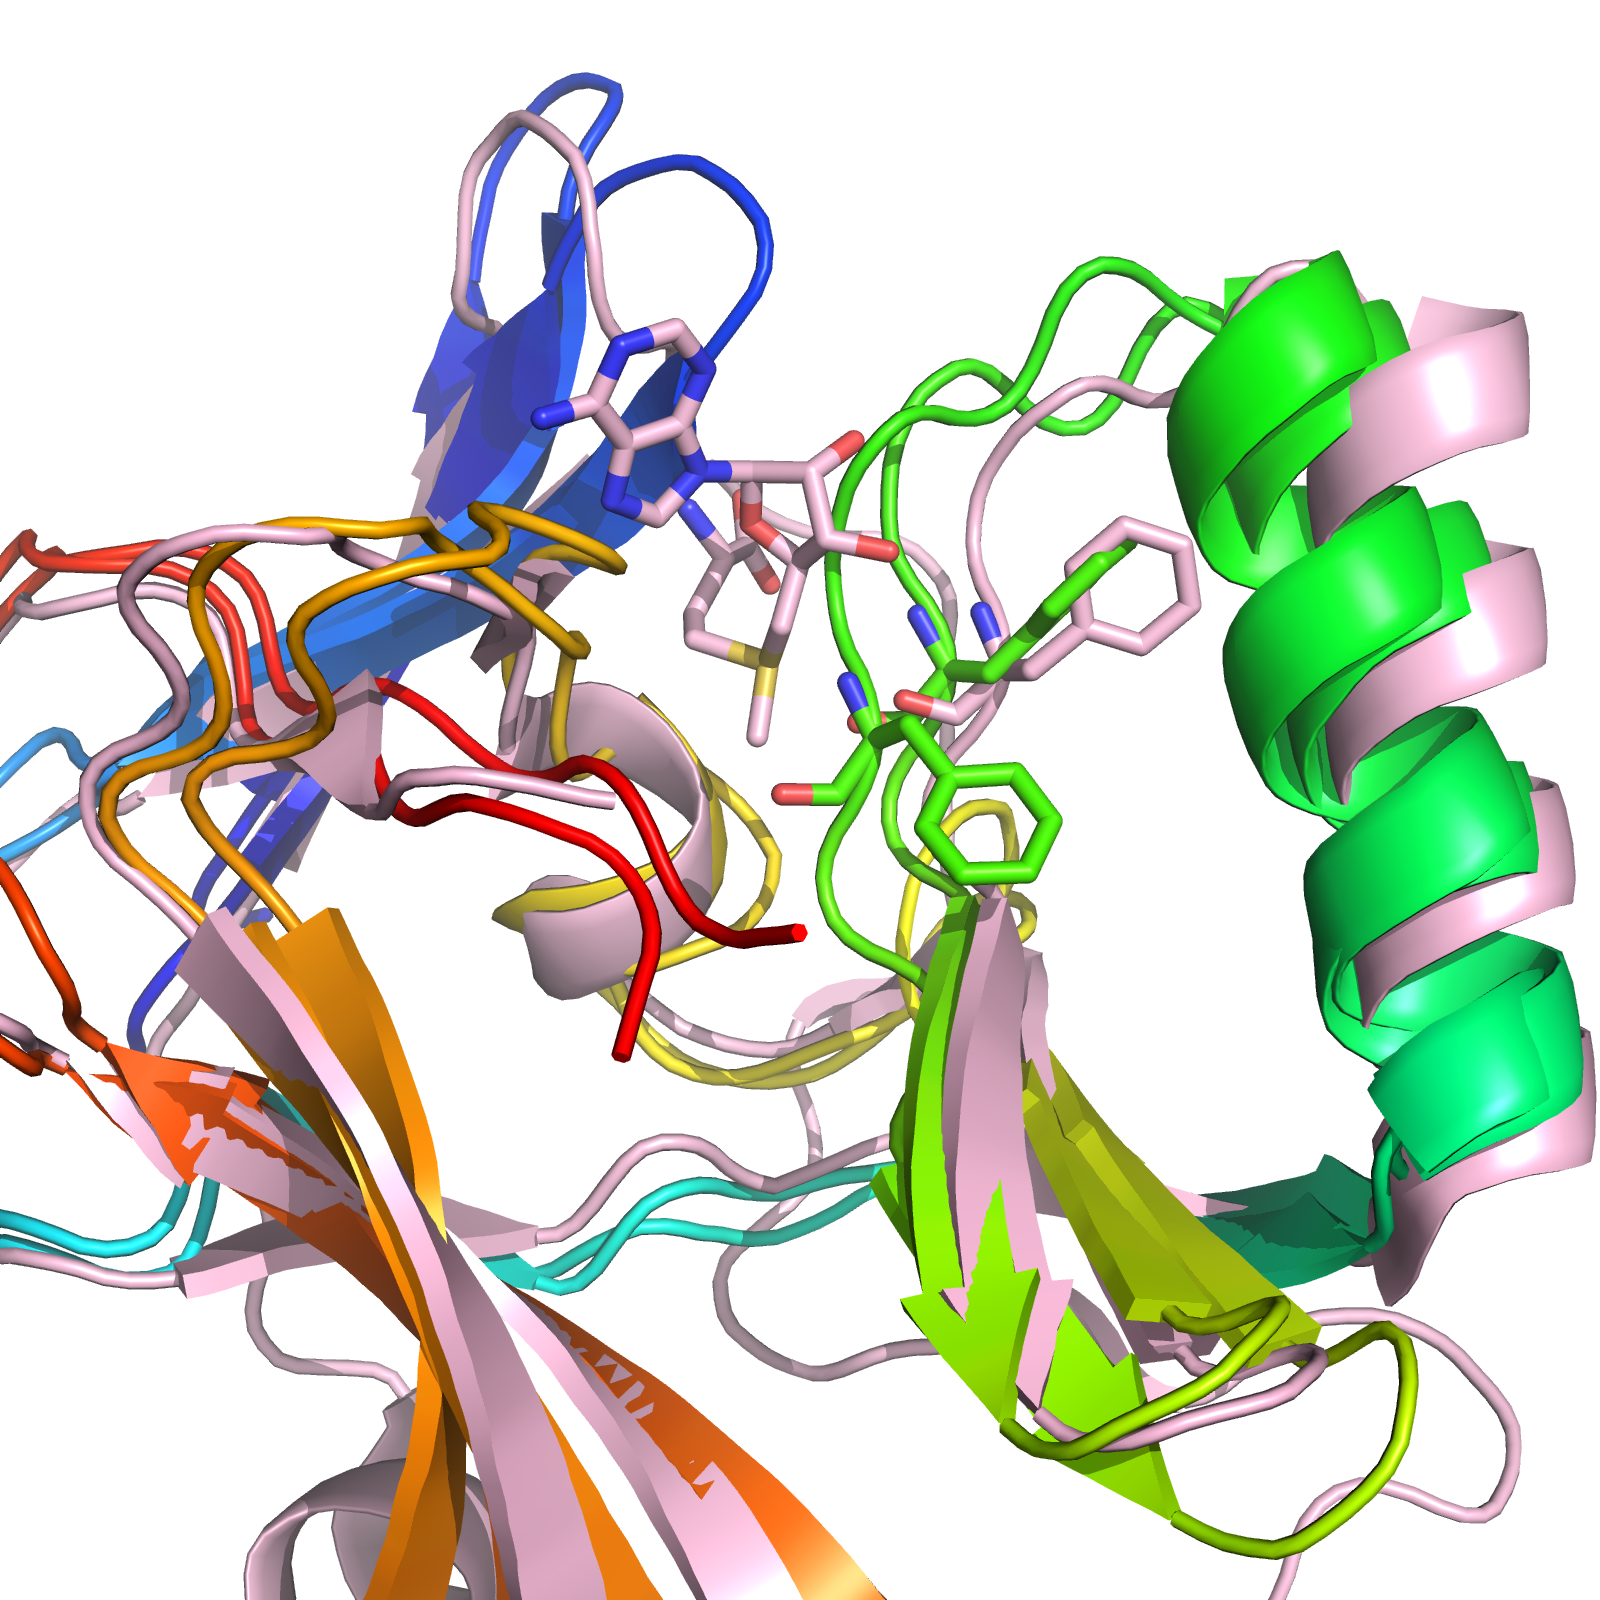
\includegraphics[width=5.5cm]{figures/NSD1_pdb.png}
}

\subfigure[]{
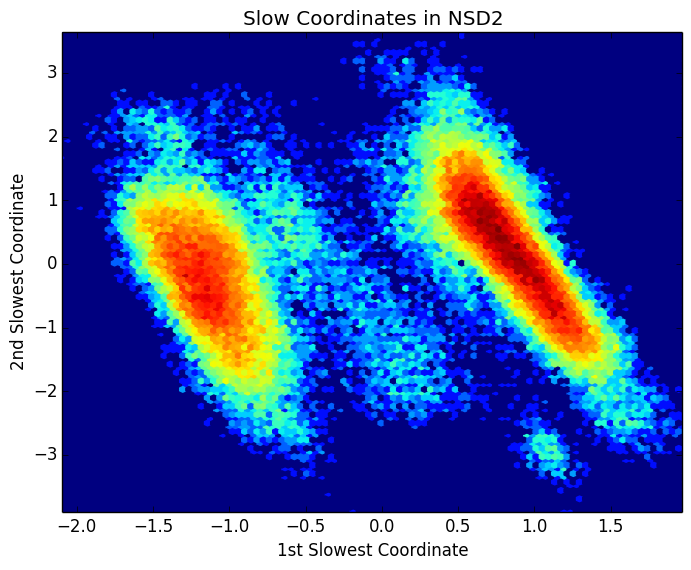
\includegraphics[width=5.5cm]{figures/NSD2_tics.png}
}
\subfigure[]{
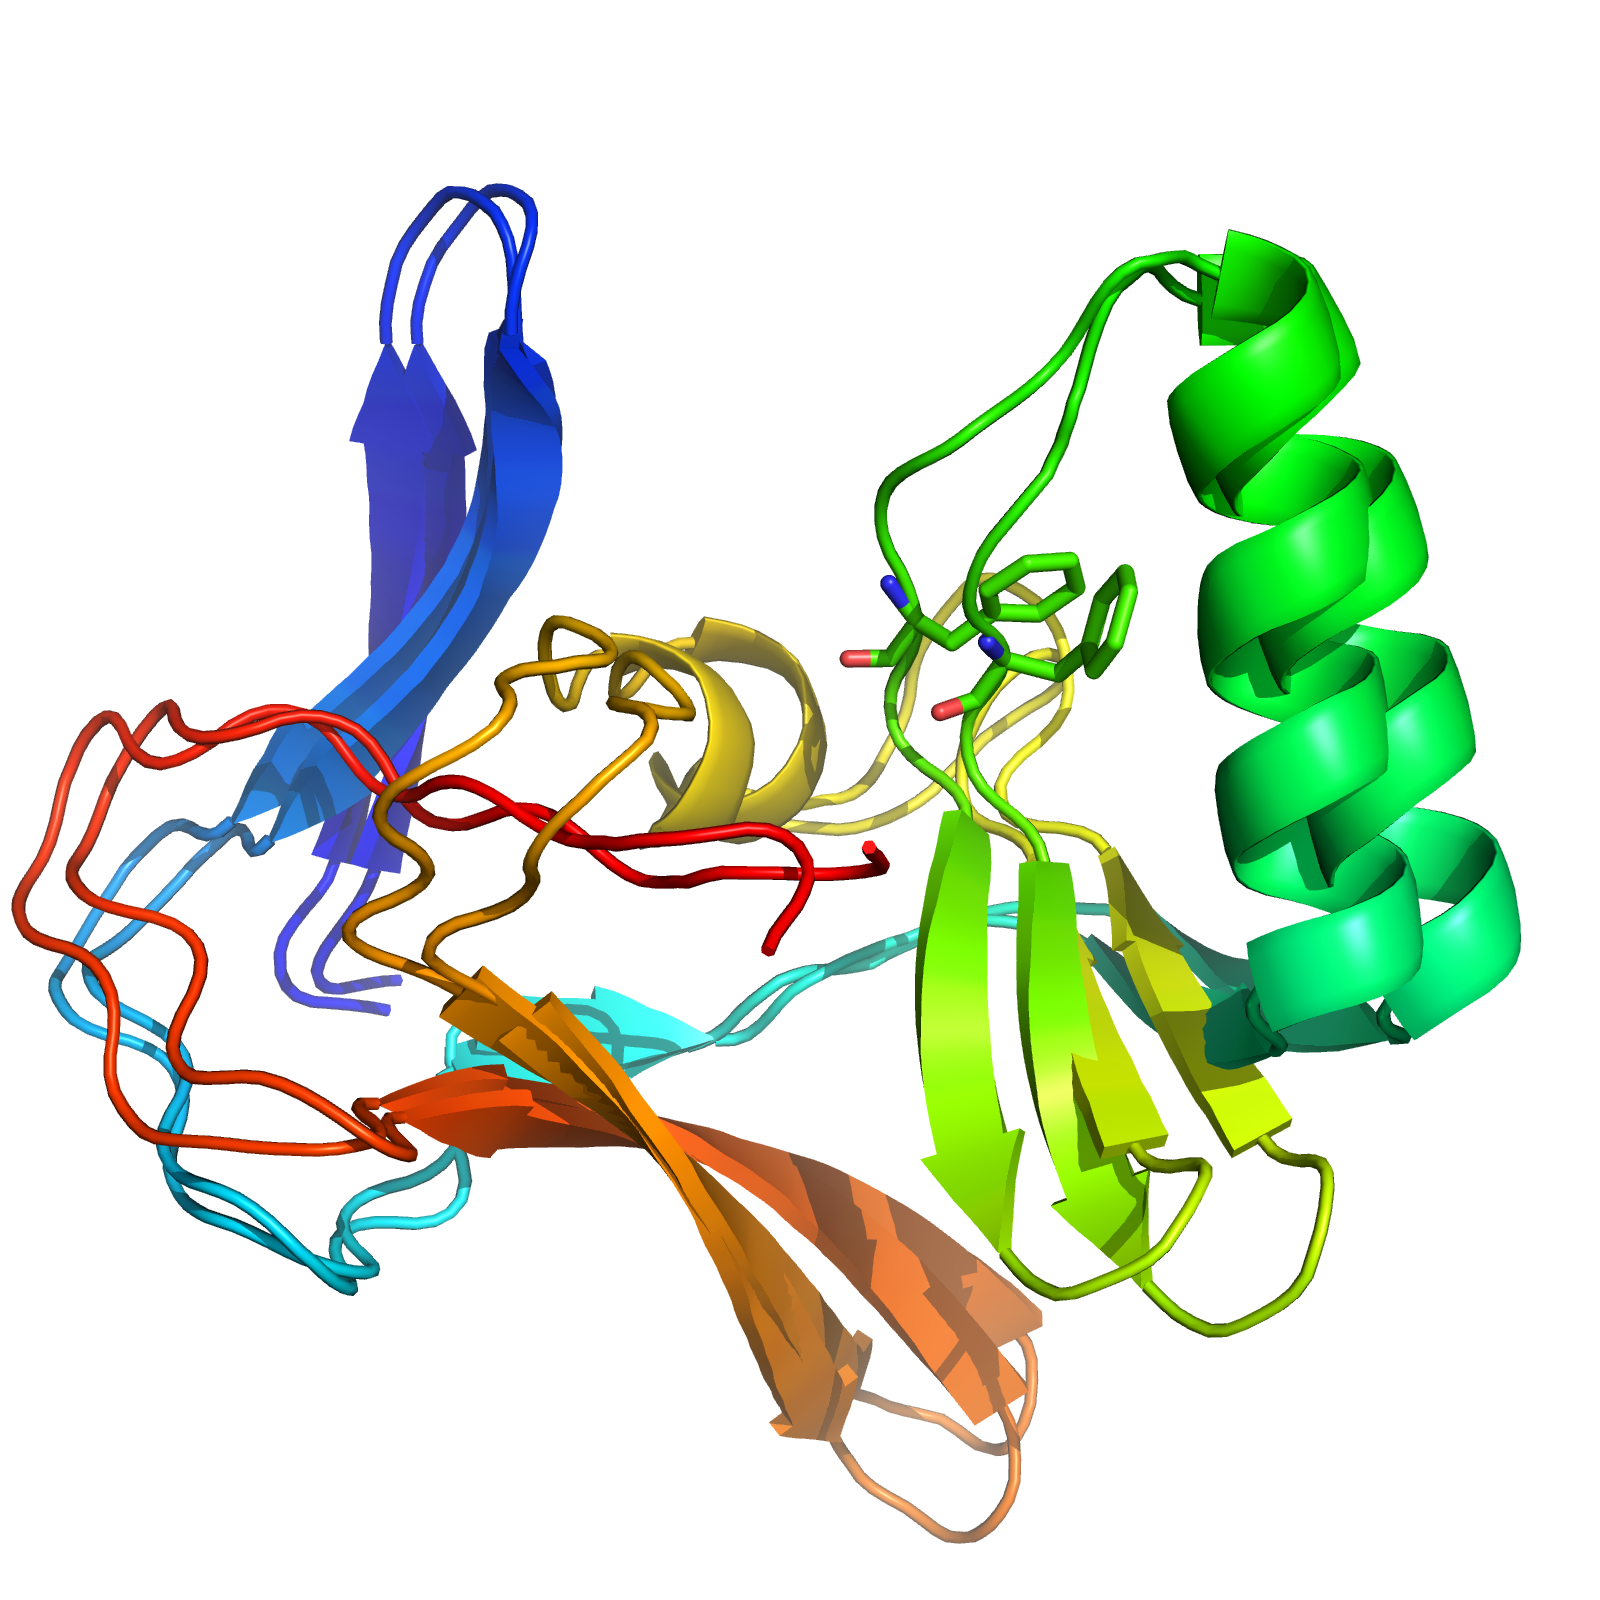
\includegraphics[width=5.5cm]{figures/NSD2_pdb.png}
}

\caption{
Maps of the two slowest coordinates of SETD2 (a), NSD1 (c), and NSD2 (e) show multiple conformational states observed in simulations at the ~$10 \mu s$ timescale.  Comparison of the observed states (b: SETD2, d: NSD1, e: NSD2) indicate conformational heterogeneity near the known SAM / sinefungin binding site--particularly in the packing of nearby aromitic side chains.  Ligand-bound crystal structures show similar conformational states.  SETD2 bound to SAH (b: cyan) adopts a TYR-up orientation (PDB:4H12), while SETD2 bound to sinefungin (b: pink) adopts a TYR-down orientation (PDB:4HMU).  NSD1 bound to SAM (d: pink) adopts a PHE-up conformation (PDB: 3OOI).  In all three systems, simulations suggest the presence of both conformations in solution, suggesting that predictive models of binding affinity and selectivity will require careful accounting for the conformational preferences of the unbound protein.
}
\label{figure:MSM}
\end{figure}



In 




\end{document}
